\chapter{Introdução}
\label{chap:introducao}

O problema de busca de rotas otimizadas, amplamente conhecido na ciência da computação como \textit{pathfinding}, representa uma das categorias mais clássicas e fundamentais dos problemas de otimização. Desde a roteirização de pacotes em redes de computadores até a navegação de veículos autônomos e a movimentação de personagens em jogos digitais (\textit{NPCs}), a necessidade de deslocar um agente de um ponto de origem a um ponto de destino gastando a menor quantidade de recursos possível é um desafio constante e de alta relevância prática.

No escopo deste trabalho, o problema de otimização escolhido consiste na navegação espacial em um ambiente bidimensional (malha ou \textit{grid}) onde o custo de deslocamento não é homogêneo. Diferentemente de cenários simplificados onde a distância métrica é o único fator limitante, o ambiente modelado apresenta diferentes tipos de superfícies e obstáculos, cada um impondo uma penalidade distinta ao deslocamento do agente, definida como ``Custo de Energia''. O objetivo central do problema é encontrar um caminho válido que conecte a origem ao destino minimizando o somatório total de energia gasta ao longo do trajeto.

Para ilustrar, analisar e testar a resolução matemática deste problema, foi desenvolvida uma aplicação interativa estruturada como um jogo de quebra-cabeça (\textit{puzzle}) em 2D. A topologia do ambiente é composta por terrenos modulares, cujos pesos foram definidos da seguinte forma:

\vspace{0.5cm}
\begin{table}[h]
\centering
\begin{tabular}{llc}
\toprule
\textbf{Tipo de Terreno} & \textbf{Características} & \textbf{Custo de Energia} \\
\midrule
Grama & Superfície plana e de fácil locomoção & 1 \\
Morro & Elevação que exige maior esforço físico & 2 \\
Água & Superfície densa e de movimentação lenta & 3 \\
Parede & Superfície intransponível & $\infty$ \\
\bottomrule
\end{tabular}
\caption{Tabela de custos associados aos terrenos do ambiente virtual.}
\label{tab:custo_enegia}
\end{table}
\vspace{0.5cm}

\begin{figure}[H]
    \centering
    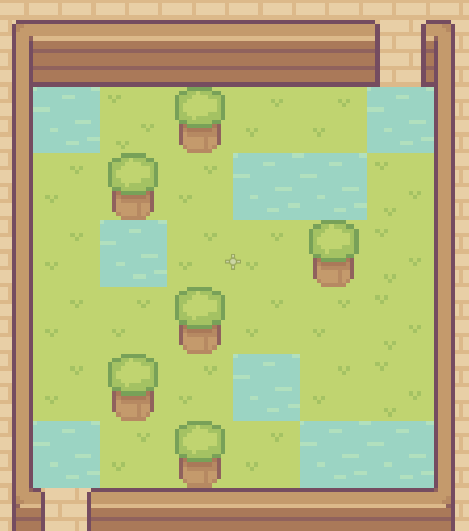
\includegraphics[width = 0.5\textwidth]{figuras/grid_game.png}
    \caption{\textit{Grid} do Jogo}
    \label{fig:gird_game}
    \fonte{Elaborado pelos autores (2026).}
\end{figure}


A principal contribuição e diferencial da modelagem proposta é a análise comparativa entre a intuição humana e a precisão algorítmica. Na aplicação desenvolvida, o usuário humano é desafiado a traçar, de forma manual e baseada em sua percepção visual, o caminho que julga consumir a menor quantidade de energia. Após a tentativa humana, o sistema computacional resolve o mesmo mapa utilizando o algoritmo heurístico A* (A-Estrela), revelando a rota matematicamente ótima (\textit{gabarito}). 

Essa abordagem interativa permite comparar a intuição do jogador contra a precisão matemática da máquina. Ao medir a diferença de custo entre a rota escolhida no 'olhômetro' pelo humano e o gabarito perfeito gerado pelo A*, o trabalho prova na prática por que algoritmos de busca são fundamentais para não desperdiçar recursos em problemas de otimização.
